%
% Since this is a ``report'', the topmost level of hierarchy is
% ``Chapter'', not section as you may be used to. Chapters are
% enumerated starting from 1, so Sections are 1.1, Subsections are
% 1.1.1, subsubsections don't get numbers. (You can change that, if
% you want them to be called 1.1.1.1)
%
\chapter{Policy Inference with Gaussian Policy Estimate}\label{chapt:gauss_policy}

    The multi-agent system presented in this thesis is modeled with two agents, the controllable agent \agent{1} and the
    uncontrollable agent \agent{2}. Explicitly, these agents exist within a hidden-parameter \ac{MDP}, where the hidden
    parameter is the action distribution, policy, of \agent{2}. If \agent{1} is given a task, it can only robustly plan
    for this task when it has an accurate estimate of how \agent{2} will act. Determining the action distribution of an
    uncontrollable agent given its current state is known as \textit{policy-inference}. The following definitions
    formally present a hidden policy in \iac{MDP}.

    After defining the hidden-parameter MDP, this chapter presents an inference method that uses Monte-Carlo integration
    of policy parameters sampled from a multivariate distribution. We'll use \ac{SGA} to improve the log-likelihood of
    an observed set of data given a policy parameterization. Section \ref{sec:policy_parameterization} details a
    $Q$-function approximation which is used to form a softmax policy like in \cite{something}, also known as a Boltzman
    \cite{something-else} and a Gibbs \cite{another} policy.

    Finally, the algorithm
    will be tested in a single-agent grid world before demonstrating a two agent example in Chapter
    \ref{chapt:proactive_inference}. We could increase the number controllable and uncontrollable agents but a two agent
    example sufficiently demonstrates the algorithm framework.


\section{Hidden-parameter MDP}\label{sec:hipmdp}
    \begin{definition}\label{def:hipmdp}
        The interaction between two agents is captured by a hidden-parameter \ac{MDP},
        \[
            \mathcal{M} = (S, A_1 \times A_2, R, T, \policy{2}, I_0 , \gamma)
        \]
        with the tuple defined as in \cite{Sugiyama2015StatisticalRL} plus the hidden parameter, $\policy{2}$:
        \begin{itemize}
                \item $S \equiv (S_1 \times S_2)$ is a set of joint states with cardinality $0 < |S| \leq \infty$ .
            \item $A_1\times A_2$ is a finite set of actions, where $A_1$ is the set \agent{1} can execute and $A_2$ is
                the set available to \agent{2}.
            \item $R: S\times A_1 \rightarrow \reals$ is the real-valued state-action reward function given to the
                controllable agent.
            \item $T: S\times (A_1\times A_2)\rightarrow \dist(S)$ is the probabilistic state transition function
                $ T(s'| s, (a_1,a_2)) $ which yields the probability of reaching state $\textnormal{s}'$ after both
                agents take action pair $(\text{a}_1,\text{a}_2)$ at the state $\textnormal{s}$.
            \item $\policy{2} : S \rightarrow \dist(A_2)$ The distribution of \agent{2}\!'s actions given a
                state. The probability of each action is $\policy{2}(a_2|s),\ \forall\ a_2 \in A_2$.
            \item $I_0 \in \dist(S)$ is the initial state distribution.
            \item $\gamma$ The discounting factor $(0,1)$.
        \end{itemize}
    \end{definition}

    \noindent
    This definition also leads us to a couple pivotal assumptions in this work:

    \begin{assumption}
        The state-action transition function $T(\cdot)$, is known.
    \end{assumption}

    \begin{assumption}
        The unknown policy of \agent{2}, $\policy{2}$, produces a stationary- and ergodic-stochastic process; the policy
        is Markovian.
    \end{assumption}

    Given that \agent{1} takes some action $a_1$, the distribution of next states is
    \begin{equation}\label{eq:true_state_action_trans_prob}
        P(s'| s, a_1) = \sum_{a_2\in A_2} T\left(s'|s, (a_1,a_2)\right)\policy{2}(a_2|s).
    \end{equation}

    \noindent
    With this model, the true probability of a future state $s'$ given the current state $s$ is
    \begin{equation}\label{eq:true_state_trans_prob}
        p(s'|s) = \sum_{a_1, a_2 \in A} T \left(s'|s, (a_1,a_2)\right)\policy{2}(a_2|s)\policy{1}(a_1|s),
    \end{equation}

    \noindent
    where, for simplicity, this report uses identical action sets, $A_1 \equiv A_2 \equiv A$. Finally, the \ac{MDP}
    formed by the tuple $(S, A_1 \times A_2, R, T, \policy{2}, I , \gamma)$ will be referred to as $\mathcal{M}$. Let's
    now justify the algorithm used for policy inference.

    \todo[inline,color=green]{Potentially explain the difference between HIP-MDP and POMDP? }


\section{Policy Inference Objective Function}\label{sec:policy_obj}
    Consider that the main goal of \agent{1} is to complete its task and a secondary goal is to infer the policy of
    \agent{2}. The estimate of \agent{2}'s policy, $\estimate{\policy{}}_2$, is parameterized by a vector \vect{\theta}.
    Therefore, the estimated probability of a state transition is
    \begin{equation}\label{eq:est_state_trans_prob}
        q(s'|s, \vect{\theta}) = \
            \sum_{a_1, a2 \in A}P(s'|s,(a_1,a_2))\estimate{\policy{}}_2(a_2|s,\vect{\theta})\policy{1}(a_1|s).
    \end{equation}

    As the \agent{2} moves through $S$, the robot agent can observe the outcomes of \agent{2}'s actions, and build a set
    of observed state sequences.
    \begin{definition}\label{def:traj}
        A trajectory $\tau$ is a sequence of joint states $s=(s_1, s_2)$ with time-step index $t$,
        \[
        s^{(0)}, s^{(1)}, \ldots , s^{(t)}, \ldots , s^{(|\tau|)};\ 0 \leq t \leq |\tau|.
        \]
    \end{definition}

%   \noindent
%   The action-sequence of \agent{1} can be recorded for a trajectory, but the action-sequence for \agent{2} is
%   unobservable. Therefore, the state-\textit{outcome} sequence will be represented as
%   \[
%   \big((s_1,s_2)(a_1, o_1)\big)^{(t)}, \big((s_1,s_2)(a_1, o_1)\big)^{(t+1)} \ldots ;\ 0 \leq t \leq |\tau|.
%   \]


    We'll define the probability of a trajectory as the joint probability of each set state-transition tuple for each of
    the two distributions, $p$ and $q$:
    \begin{align*}
        p(\tau) &= \prod_{t=1}^{|\tau|}p\left( s^{(t)}| s^{(t-1)} \right), \\
        q(\tau|\vect{\theta}) &= \prod_{t=1}^{|\tau|}q\left(s^{(t)}| s^{(t-1)}, \vect{\theta}\right).
    \end{align*}

    \noindent
    By using the parameter \paramVec, $q(\tau,\paramVec)$ is the probability of replicating a trajectory given the
    parameterization. We'll sample a set of trajectories and build an observed demonstration set, $\tau_d \in D$.

    \begin{assumption}
        The observed demonstration set, D, is sampled i.i.d. from the set of all possible demonstrations $\mathcal{D}$.
    \end{assumption}

    The best inference of an environmental policy has a high likelihood of replicating the trajectories in $D$.
    \begin{lemma}\label{lemma:obj_fun_equiv}
        Minimizing the \ac{KLD} of the replica distribution from the observed trajectory distribution is equivalent to
        maximizing the log-likelihood of the observed state sequences given a parameterized policy, With a fixed policy
        for \agent{1}, $\policy{1}$,
        \begin{equation*}
            \argmax_{\paramVec} \logLike(\paramVec; \policy{1}) = \argmin_{\paramVec} \text{KL}(p||q_{\paramVec}).
        \end{equation*}
    \end{lemma}

    \begin{proof}
        Consider a pair of stationary policies for the two agents, $\policy{1}$ and $\policy{2}$. The induced Markov
        chain is $M_{\policy{1}, \policy{2}}$. Let $p$ be the probability distribution of paths in the chain
        $M_{\policy{1}, \policy{2}}$. Let $q_{\paramVec}$ be the probability distribution of paths in the chain
        $M_{\policy{1}, \estimate{\policy{}}_2}$. The \ac{KLD} from $q_{\paramVec}$ to $p$ is
        \begin{equation*}\label{eq:traj_kl_div}
            \text{KL}(p || q_{\paramVec}) = \sum_{\traj_d \in D} p(\traj_d) \ln \left( \frac{p(\traj_d)}
                                                {q(\traj_d|\paramVec)} \right)\
                = \sum_{\traj_d \in \calD} P(\traj_d|D) \ln \left( \frac{P(\traj_d|\calD)}
                                                {P(\traj_d|\policy{1},\paramVec)} \right),
        \end{equation*}

        \noindent
        where $P(\traj_d|D)$ is the maximum likelihood probability of the state sequence, and
        $P(\traj_d|\policy{1},\paramVec)$ is the probability of obtaining that state sequence by our inferred policy
        that is parameterized by the vector \paramVec.

        Minimizing the deviation of $q_{\paramVec}$ from $p$ is equivalent to maximizing the expectation of the
        observing $D$, given that the environment actions are distributed as $\policy{2}(s; \paramVec)$:
        \begin{equation}\label{eq:min_kld}
            \begin{aligned}
                \argmin_{\paramVec}(\text{KL}(p || q_{\paramVec})) & = \
                    \argmin_{\paramVec}\left(\sum_{\traj_d \in  \calD}\!  P(\traj_d|\calD)
                    \ln\left(\frac{P(\traj_d|\calD)}{P(\traj_d|\policy{1},\paramVec)}\right)\right)\\
                & = \argmin_{\paramVec}\left(\sum_{\traj_d \in D} P(\traj_d|D) \ln(P(\traj_d|D)) -
                    P(\traj_d|D) \ln\left(P(\traj_d|\policy{1},\paramVec)\right)\right)\\
                & = \argmax_{\paramVec}\left(\sum_{\traj_d \in \calD}\!  P(\traj_d|\calD)
                    \ln\left(P(\traj_d|\policy{1},\paramVec)\right)\right)\\
                & = \argmax_{\paramVec}\expectation{P(\traj_d|\calD)} {\ln(P(\traj_d|\policy{1},\paramVec))} \\
                &\approx \argmax_{\paramVec} \sum_{\traj_d \in D}  \ln(P(\traj_d|\policy{1},\paramVec))\\
                & =\argmax_{\paramVec} \logLike(D|\policy{1},\paramVec)
            \end{aligned}
        \end{equation}

        \noindent
        where we estimate the expectation using the empirical mean. We will write the final line of Eq.
        \ref{eq:min_kld} as $\logLike(\paramVec; \policy{1})$ for compactness and consistency with Lemma
        \ref{lemma:obj_fun_equiv}.

    \end{proof}

    For the rest of this report, lets assert that an optimal parameter exists.
    \begin{assumption}\label{assump:opt_policy_err}
        There exists an optimal parameter vector that can represent the true distribution of $\policy{2}(s)$ to within a
        threshold $\xi$, given that a set of basis functions are properly defined;
        \[
        \exists\ \optimal{\paramVec}\ \big|\ \Big| \OneNorm{\estimate{\policy{}}_2(s;\optimal{\paramVec})} -
            \OneNorm{\policy{2}(s)} \Big| \leq \xi.
        \]
    \end{assumption}

    \noindent
    The $\mathsf{L_1}$-norm of a policy, $\OneNorm{\policy{}(s)} = \sum_{s \in S}\sum_{a \in A}\policy{}(a|s)$, is a
    measurable distance unlike \ac{KLD}; $\text{KL}(p||q) \neq \text{KL}(q||p)$. For all following experiments, we'll
    use the absolute difference of $\mathsf{L_1}$-norm's to compare two policies.

    We are now ready to discuss the inference procedure used to identify the $\estimate{\policy{}}_2(s,
    \estimate{\paramVec})$ that maximizes the R.H.S of Lemma \ref{lemma:obj_fun_equiv}.


\subsection{Gaussian Distribution of Policy Parameters}\label{sec:gauss_policy}

    After a data set of trajectories, $D$, has been collected, \agent{1} needs to maximize $\logLike(D|\paramVec)$,
    which is the log-likelihood of the dataset when \policy{2} is parameterized by \paramVec. Let $\estimate{\paramVec}
    = [ \paramElem]_{w=1}^W$ be a vector of independently sampled random variables with Gaussian distributions
    $\mathcal{N}(\mu_w, \nu_w)$. The variance, $\nu_w^2$, will capture the uncertainty of $\paramElem$ in the inference
    from dataset $D$.

    We denote $\rho_w = (\mu_w, \nu_w)$ as the tuple of mean and variance for $\paramElem$ and denote $\rho
    =\{\rho_w\}_{w=1}^W$ to be the collection of variable tuples. Given $\rho$, the probability of the demonstrations
    is
    \[
    P(D |\rho) = \int_{\paramVec } P(D|\paramVec) p(\paramVec | \rho)d\paramVec.
    \]

    \noindent
     The log-likelihood of the demonstrations can be lower-bounded using Jensen's inequality:
    \begin{equation*}
    \logLike(D|\rho ) = \log P(D|\rho)\
         = \log \left( \int_{\paramVec}P(D|\paramVec) p(\paramVec | \rho)d\paramVec \right)\ \ge \int_{\paramVec}
            p(\paramVec|\rho)\log \big( P(D|\paramVec) \big) d\paramVec.
    \end{equation*}

    \par
    Denote this lower bound as $\tilde{\logLike}(D|\rho)=\int_{\paramVec} p(\paramVec |\rho) \log P(D|\paramVec)
    d\paramVec$. This is the lower bound on the objective function derived in Eq. \ref{eq:min_kld}! By taking
    derivative of $\tilde{\logLike}(D|\rho)$ with respect to $\rho$, we obtain the gradient of the objective function:
    \begin{equation}\label{eq:gradLogLike}
        \begin{aligned}
            \nabla_\rho \tilde{\logLike}(D|\rho)) & =
                \int_{\paramVec}\nabla_\rho p(\paramVec|\rho) \log P(D|\paramVec)d\paramVec\\
            & = \int_{\paramVec}[ p(\paramVec|\rho) \nabla_\rho \log p(\paramVec|\rho) ] \log P(D|\paramVec)d\paramVec\\
            &\approx \frac{1}{m} \sum_{ i=1}^m \left[\nabla_\rho \log P(\paramVec^{(i)}|\rho) \right] \log
                P(D|\paramVec^{(i)})
        \end{aligned}
    \end{equation}

    \noindent
    where $\paramVec^{(i)}$, $i=1,\ldots, m$ are samples generated from the multi-variant Gaussian distribution with
    mean $\vect{\mu} = [\mu_1,\ldots, \mu_W]^\top$ and covariance matrix $\mbox{diag}\left(\nu_1,\ldots, \nu_W\right)$.
    Let $\vect{\nu}$ be an equivalent representation for $\mbox{diag}\left(\nu_1,\ldots, \nu_W\right)$. Each sampled
    parameter element, $\paramElem^{(i)}$, has probability:
    \[
        P(\paramElem^{(i)} | \rho_{\paramIdx}) = \frac{1}{\sqrt[]{2\pi \sigma_w^2}}\exp
            \left( -\frac{(\theta_w^{(i)}-\mu_w)^2}{2\sigma_w^2} \right).
    \]

    \par
    The bracketed gradient in the last line of Eq. \ref{eq:gradLogLike} with respect to each element of \vect{\mu} and
    $\vect{\nu}$ are:
    \[
    \nabla_{\mu_{\paramIdx}}\log P(\paramElem^{(i)} | \rho_{\paramIdx}) =
        \frac{\paramElem^{(i)} - \mu_{\paramIdx}}{\nu_{\paramIdx}^2},\ \text{and}
    \]
    \[
    \nabla_{\nu_{\paramIdx}}\log P(\paramElem^{(i)} | \rho_{\paramIdx}) = \frac{(\paramElem^{(i)} - \mu_{\paramIdx})^2 -
        \nu_{\paramIdx}^2}{\nu_{\paramIdx}^3}.
    \]
    Note that superscripts enclosed in parenthesis represent sample indexes, e.g., the $i$-th sample of parameter
    element $w$ is $\paramElem^{(i)}$. All purely numeric superscripts are exponents.

    We can obtain the optimal collection of parameters $\optimal{\rho}= \argmax_{\rho} \tilde{\logLike{}}(D|\rho)$ by
    performing gradient ascent on the parameter distributions, $\rho = (\vect{\mu}, \vect{\nu})$. The policy
    parameterized by $\optimal{\estimate{\paramVec}} \sim \mathcal{N}(\optimal{\vect{\mu}}, \optimal{\vect{\nu}})$ is
    $\estimate{\policy{}}_{2}(s; \optimal{\estimate{\paramVec}})$ and it maximizes the log likelihood of the
    demonstration set $D$. The log likelihood of observed demonstrations for a given $\paramVec^{(i)}$ can be computed
    as
    \begin{align*}
        \log P(D|\paramVec^{(i)}) & = \sum_{\tau_d \in D} \log P\left(\tau_d |\paramVec^{(i)}\right)\\
        & = \sum_{d=1}^{\abs{D}} \left[ \sum_{t=0}^{\abs{\tau_d}-1} \log P \left(s^{(t+1)}|(s, a_1, o_2)^{(t)}\right) +
            \sum_{t=0}^{\abs{\tau_d}-1} \log \policy{2}\left(o_2^{(t)}|s^{(t)}; \paramVec^{(i)}\right) \right]\\
        & = \sum_{s\in S}\sum_{o_2\in A} C(s, o_2) \log \policy{2}\left(o_2|s; \paramVec^{(i)}\right) + Const.
    \end{align*}
    \todo[inline, color=green]{Note the change between this equation and the CDC draft. I have dropped $a_1$ from
    $C(\cdot)$ because the \agent{1} and \agent{2} take actions simultaneously.}
    Above, $C(s, o_2)$ is the number of times the state action pair $(s,o_2)$ is observed from in $D$. The constant
    term, $Const =\sum_{d=1}^{\abs{D}} \sum_{t=0}^{\abs{\tau_d}-1} \log P\left(s^{t+1}|(s ,a_1,o_2)^{(t)}\right)$, is
    independent of $\paramVec^{(i)}$ and can be precomputed for a demonstration $D$. The observed action outcome at
    time-step $t$ is $o_2^t$, which is the only action information available in a trajectory, per Definition
    \ref{def:traj}. If a trajectory fragment $(s_1, s_2)^{(t)}, (s_1', s_2')^{(t+1)}$ is observed, the action of the
    controllable agent, $a_1^{(t)}$, is known but the uncontrolled action, $a_2^{(t)}$, is not. Therefore $o_2^{(t)}$ is
    assigned to be the nominal motion that causes the transition $s_2^{(t)} \rightarrow s_2^{(t+1)}$ in the graph of
    $\mathcal{M}$.

    \todo[inline,color=green]{talk to Prof. Fu about the remark, below. I'm not automatically dropping basis functions,
    it would be hard to define that for only a single action at a kernel, but I could mask the parameter value to always
    be zero. I'm unsure if we actually want to do this. For the two-stage algorithm in Chapter
    \ref{chapt:proactive_inference}, these values might simply have had no data near them. }
    \begin{remark}
        If the policy does not depend on a basis function $\phi_w$, then the mean $\mu_w=0$ and the basis function will
        be removed from the set of basis function as well as the corresponding parameter $\nu_w$.
    \end{remark}

\subsubsection{Gradient Ascent}

    Using the gradient defined in Eq. \ref{eq:gradLogLike}, for each iteration $n$ we sample a set of $m$ parameter
    vectors, and update the distribution parameters on each iteration:
    \begin{equation}\label{eq:gradient_update}
        \begin{aligned}
            \dot{\vect{\mu}}_n & \leftarrow \eta\dot{\vect{\mu}}_{n-1} \lambda\nabla_{\vect{\mu}_n}
                                    \tilde{\logLike}(D|\rho_n)\\
            \vect{\mu}_{n+1} & \leftarrow\ \vect{\mu}_n + \dot{\vect{\mu}}_n\ \text{and}\\
            \dot{\vect{\nu}}_n & \leftarrow \eta\dot{\vect{\nu}}_{n-1} \lambda\nabla_{\vect{\nu}_n}
                                    \tilde{\logLike}(D|\rho_n)\\
            \vect{\nu}_{n+1} & \leftarrow \vect{\nu}_n + \dot{\vect{\nu}}_n.
        \end{aligned}
    \end{equation}

    \noindent
    The stepsize parameter, $\lambda$, limits the rate of change of the distribution moments, and the velocity memory,
    $\eta$ helps the iteration bootstrap itself through local minimums as suggested by \cite{kingma2014adam}. The ``velocity'' of each gradient is stored in
    $\dot{\vect{\mu}}_n$ and $\dot{\vect{\nu}}_n$, respectively.

\subsubsection{Algorithm Termination}\label{sec:policy_infer_terminate}

    In general, the gradient ascent should be terminated at some final iteration $N$ when the update to the parameters
    no longer improves
    $\tilde{\logLike}(D|\rho)$. This log-likelihood is bounded,
    \[
    \log P(D|\paramVec^{(i)}) \leq 0,\  \forall \paramVec \in \varTheta,
    \]
    where $\varTheta$ is the domain of the parameter vector. Due to the nature of sampling, there is no guarantee that
    for every iteration $\logLike(D|\rho_{n+1})> \logLike(D|\rho_n)$. Therefore, we'll use a moving average of the past
    $\Lambda$ log-likelihoods,
    \[
    \mathsf{HIST}(\logLike_n)=\frac{1}{\Lambda}\sum_{v=0}^{\Lambda-1}\logLike(D|\rho_{n-v}).
    \]
    We record the previous value of the moving average, $\mathsf{HIST}(\logLike_{n-1})$, and if the improvement in the
    moving average is below a defined threshold,
    \[
    \Delta\mathsf{HIST}(\logLike_n) = \mathsf{HIST}(\logLike_n) - \mathsf{HIST}(\logLike_{n-1}) \leq \zeta,
    \]
    the algorithm will terminate. We'll require that at least $N$ iterations are performed before termination. Upon
    termination the mean values of $\rho_{n}$ are assigned to the parameter vecture used to build
    $\estimate{\policy{}}_{2}(s;\estimate{\paramVec}),\ \estimate{\paramVec} \leftarrow \vect{\mu}_n.$

\subsection{Policy Iteration Preliminaries}\label{sec:policy_iteration_preliminaries}
    The parameterization for \policy{2} requires a an understanding of how a reward function, $R$, influences the
    optimal action distribution at a state $s$. Although we do not wish to learn the reward function of \agent{2}, we
    will build approximations of the \textit{value} and \textit{state-action value} functions used by \agent{2}. These
    are often a function of a reward function.

\subsubsection{Value Functions}
    Following \cite{hernandez2012adaptive} and \cite{Sugiyama2015StatisticalRL}, the value of a state $s$ is defined as
    the expectation over all discounted future rewards that could be earned from $s$. If any agent, \agent{i}, follows a
    policy \policy{i}:
    \[
    V_{\policy{i}}(s) = \expectation{\policy{i}}{\sum_{t=0}^{\infty} \gamma^t R\left((s,a_i)^{(t)}\right)
        \bigg|s^{(t)}=s}.
    \]
    The subscript in $\expectation{\policy{i}}{\cdot}$ means that the expectation is taken over the Markov chain, which
    is induced by \agent{i} playing policy $\policy{i}$ in the \ac{MDP},
    \[
    V_{\policy{i}} = \expectation{\policy{i}}{R\left((s,a_i)^{(t)}\right) + \gamma V_{\policy{i}}(s^{(t+1)})}.
    \]

\subsubsection{State-action Value (Q) Functions}
    Likewise, the value of an action at a particular state is the expected discounted future reward following policy
    \policy{i}:
    \[
    Q_{\policy{i}}(s,a_i) = \expectation{\policy{i}}{\sum_{t=0}^{\infty} \gamma^t R\left((s,a_i)^{(t)}\right)
        \bigg|s^{(t)}=s, a_i^{(t)}=a_i}.
    \]

\subsubsection{Policy Solution}
    A policy $\optimal{\policy{i}}$ is said to be \textit{optimal} if it maximizes the expected total discounted reward
    from a given initial distribution $I_0$. For a deterministic policy this is,
    \[
    \optimal{\policy{i}} \leftarrow \arg\max_{\policy{i}}\sum_{s\in S} V_{\policy{i}}(s)I_0(s) .
    \]
    Methods to obtain (sub)optimal policies for the controllable agent, $\policy{1}$, will be discussed in Chapter
    \ref{chapt:policy_iteration}. This will also cover \textit{asymptotic} discount optimality from
    \cite{hernandez2012adaptive} since $\estimate{\policy{}}_2(s;\estimate{\paramVec})$ has a non-zero error from the
    truth.

\subsection{Q-function Approximation}\label{sec:policy_parameterization}
    The model of $\policy{2}(s; \paramVec)$ approximates the \textit{state-action value function}, $Q(s,a_2)$, with a
    linear-in-parameter model. Sugiyama describes this model in detail in Section 2.2.1 of
    \cite{Sugiyama2015StatisticalRL}. It is advantageous that \agent{1} does not need to learn the reward function of
    \agent{2}, but only the distribution of \agent{2}'s action given the joint state set, $\policy{2}(s),\ s\in S$. Each
    parameter element determines the weighting of a feature $\phi : S \times A_2 \rightarrow \reals$. If a total of
    $\paramLen$ features are used then \agent{2}'s \textit{Q}-function is approximated as
    \begin{equation*}\label{eq:QFuncApprox}
        Q(s,a_2) \approx \estimate{Q}(s,a_2)
            = \sum_{\paramIdx=1}^{\paramLen} \estimate{\paramSym}_{\paramIdx} \featElem(s,a_2)
            = \estimate{\paramVec}^\top \featFunc.
    \end{equation*}

    Following Chapter 3 of \cite{Sugiyama2015StatisticalRL}, we'll use \acp{GGK} because they intuitively incorporate
    any obstacles\footnotemark\ that exist in $S$ into a distance metric between a state $s$, and the center of a
    \ac{GGK}, $c$. Consider the state-graph of $\mathcal{M}$. If there are $K$ kernels, and the $l$-th kernel has center
    $c$, then the value of the kernel at a state $s$ is
    \begin{equation*}
        \kernFunc(s,\kernCent_{\kernIdx}) = \exp \left( \frac{-\text{SP}(s,\kernCent_{\kernIdx})^2}
            {2\kernStdDev^2_{\kernIdx}} \right).
    \end{equation*}

    \footnotetext{Obstacles could be considered as known sink-states in $\mathcal{M}$, and will be clarified in Sect.
                  \ref{sec:single_agent_experiment}.}

    \noindent
    The \ac{SP} between a state $s$ and the $l$-th kernel's center $c_l$ can be precomputed, and the kernel standard
    deviation, $\kernStdDev_{\kernIdx}$, determines the effective support of the kernel. The feature function is defined
    for each action, so the number of features is $W = |A| \times K$. The $w$-th feature function is
    \begin{equation}\label{eq:kernel_func}
        \featElem(s_2,a_2) = I(a_2==a_2^{(j)})\sum_{s_2'\in S_2}P\left(s_2'|s_2,a_2^{(j)}\right)
            \kernFunc(s_2',c_{\kernIdx}),
    \end{equation}

    \noindent
    where $w=j+(\kernIdx|A_2|-1)$ represents the index used for both feature-vector functions and parameter elements,
    \paramElem. Also, for each action $a_2$ the indicator function ${I(a_2==a_2^{(j)})}$ is defined as:
    \begin{equation*}
        \begin{aligned}
            I(a_2==a_2^{(j)}) & = \begin{cases}
                                      0 & \text{if}\ a_2 \neq a_2^{(j)} \\
                                      1 & \text{if}\ a_2 = a_2^{(j)}
                                  \end{cases} \\
            j & = 1, \ldots, |A_2|,
        \end{aligned}
    \end{equation*}

    \noindent
    assuming all actions are enabled from each state $s_2 \in S_2$.

    Given a $Q$-function, \cite{nachum2017bridging} represents the policy at a state as represented the softmax over all
    actions,
    \begin{equation}\label{eq:policy_model}
        \policy{2}(a_2|s) = \exp((Q(s,a_2)- V(s))/\kappa),
    \end{equation}

    \noindent
    where $V(s) = \kappa\log \sum_{a_2\in A}\exp (Q(s,a)/\kappa)$. Also, $\kappa$ is a temperature parameter. If $\kappa
    \rightarrow \infty$, the distribution $ \policy{2}(s) $ becomes uniform over $A_2$. If $\kappa \rightarrow 0$, the
    distribution $\policy{2}(s)$ becomes a Dirac Delta distribution that peaks on the action $a_2^\ast = \argmax_{a_2}
    Q(s,a_2)$. In the inference algorithm, we consider $\kappa$ as a predefined hyper-parameter in the range
    $(0,\infty)$.

    This is the model used for \policy{2} in the rest of this report. The advantage of this parameterization is that we
    have reduced the number of parameters to learn from $|S|\times A$ to $W$. We'll show that we can effectively infer a
    policy with $K \ll |S|$.

\section{Single-agent policy inference experiment}\label{sec:single_agent_experiment}
    The algorithm and parameterization presented in Sections \ref{sec:gauss_policy}-\ref{sec:policy_parameterization}
    are initially tested in a single agent environment. In this example, the states are just $s=s_2 \in xS$, and
    $\policy{1}(a_1|s)$ is dropped from Eq. \ref{eq:true_state_trans_prob}.

\subsection{Simulation environment}
    Assume that \agent{2} exists alone in a $5\times5$ grid world. In a single agent simulation, states and grid-cells
    are synonymous. The available action set is
    \[
    A = \{Empty, North, South, East, West\},
    \]
    which correspond to their motion primitives
    \[
     \{Stay, Up, Down, Right, Left\}.
    \]
    The motion resulting from an action $a_2$ is stochastic; the intended motion is actually executed with a probability
    of $0.8$, and there is a probability of $0.1$ of sliding in the two perpendicular motion directions. The exception
    is the $Empty$ action which results in a $Stay$ motion with probability $1$. The boarder of the grid-world are
    considered to be walls. If the resulting motion causes the agent to leave the grid then $Stay$ is selected, $s'=s$.
    Table \ref{table:motion_model} clarifies the motion model for the $East$ action based on the starting cell location.

    \begin{table}[h!]
    \centering
    \begin{tabular}{ c || c | c | c | c}
              & \multicolumn{4}{c}{Starting grid-cell location type}\\
        %\hline
        Resulting Motion & Middle & Right Column & Top Row & Upper Right Corner\\
        \hline
        %      &       &       &       \\
        North & $0.1$ & $0.1$ & $0.0$ & $0.0$ \\
        South & $0.1$ & $0.1$ & $0.1$ & $0.1$ \\
        East  & $0.8$ & $0.0$ & $0.8$ & $0.0$ \\
        West  & $0.0$ & $0.0$ & $0.0$ & $0.0$ \\
        Stay  & $0.0$ & $0.8$ & $0.1$ & $0.9$ \\
    \end{tabular}
    \label{table:motion_model}
    \caption{Agent motion model given attempted \textit{East} (right) action.}
    \end{table}

    The \textit{hidden} policy of \agent{2} is visualized in Fig. \ref{fig:single_agent_2_policy}. The policy is
    deterministic, $\kappa=0$, and the agent has a hidden goal of the green cell. The red cells are obstacles, are
    \textit{not} hidden, and are sink states. Arrows represent the direction an action is selected with probability $1$,
    and dots represent that the $Empty/Stay$ action is selected with probability $1$. A demonstration set $D$ is
    generated with a uniform initial distribution $s^{(0)} \sim \mathcal{U},\ \forall \traj_d \in D$. The state
    visitation count for the example $D$ is visualized in Fig. \ref{fig:single_agent_demo}

    \todo[inline]{Perhaps I need to add a \textit{Label} definition to of the HIPMDP.}
    \todo[inline]{change the color of agent \textbf{2}'s goal to yellow, to limit confusion in future sections}

    \begin{figure}[htb]
        \begin{center}
            \fbox{
                \begin{minipage}{0.5\textwidth}
                    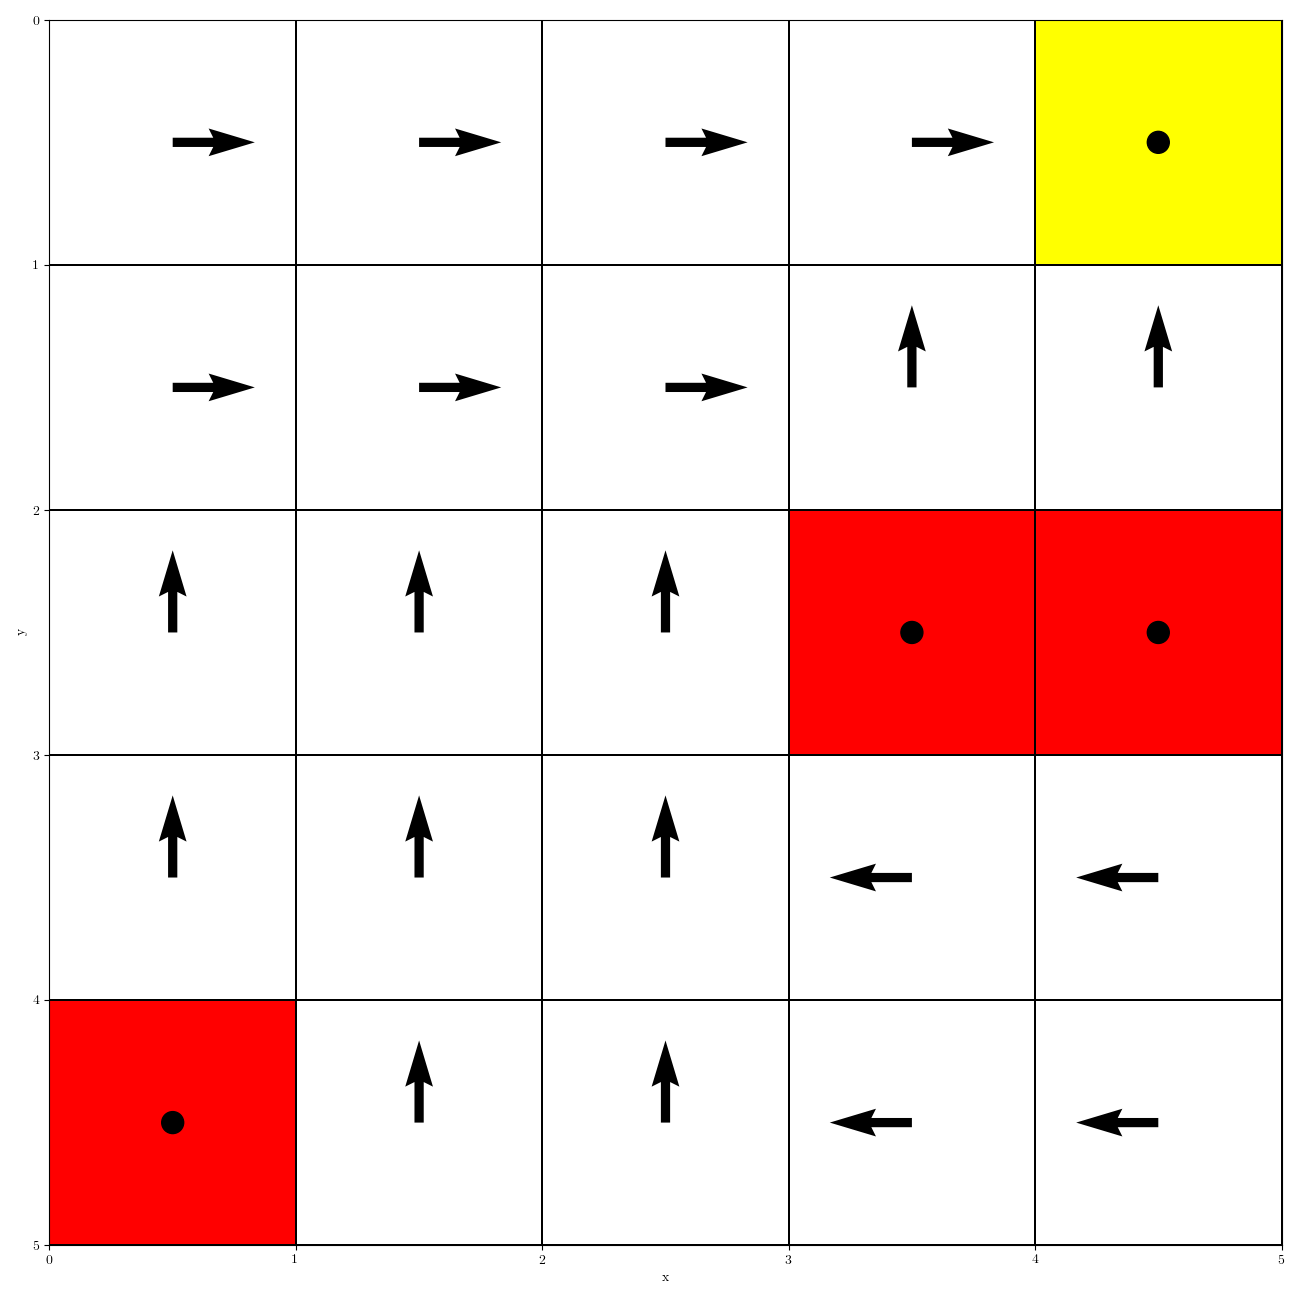
\includegraphics[width=\textwidth]{single_agent_2_policy}
                    \caption{True Policy of \agent{2}.}
                    \label{fig:single_agent_2_policy}
                \end{minipage}
                }
        \end{center}
    \end{figure}


    \begin{figure}[htb]
        \begin{center}
            \fbox{
                \begin{minipage}{0.5\textwidth}
                    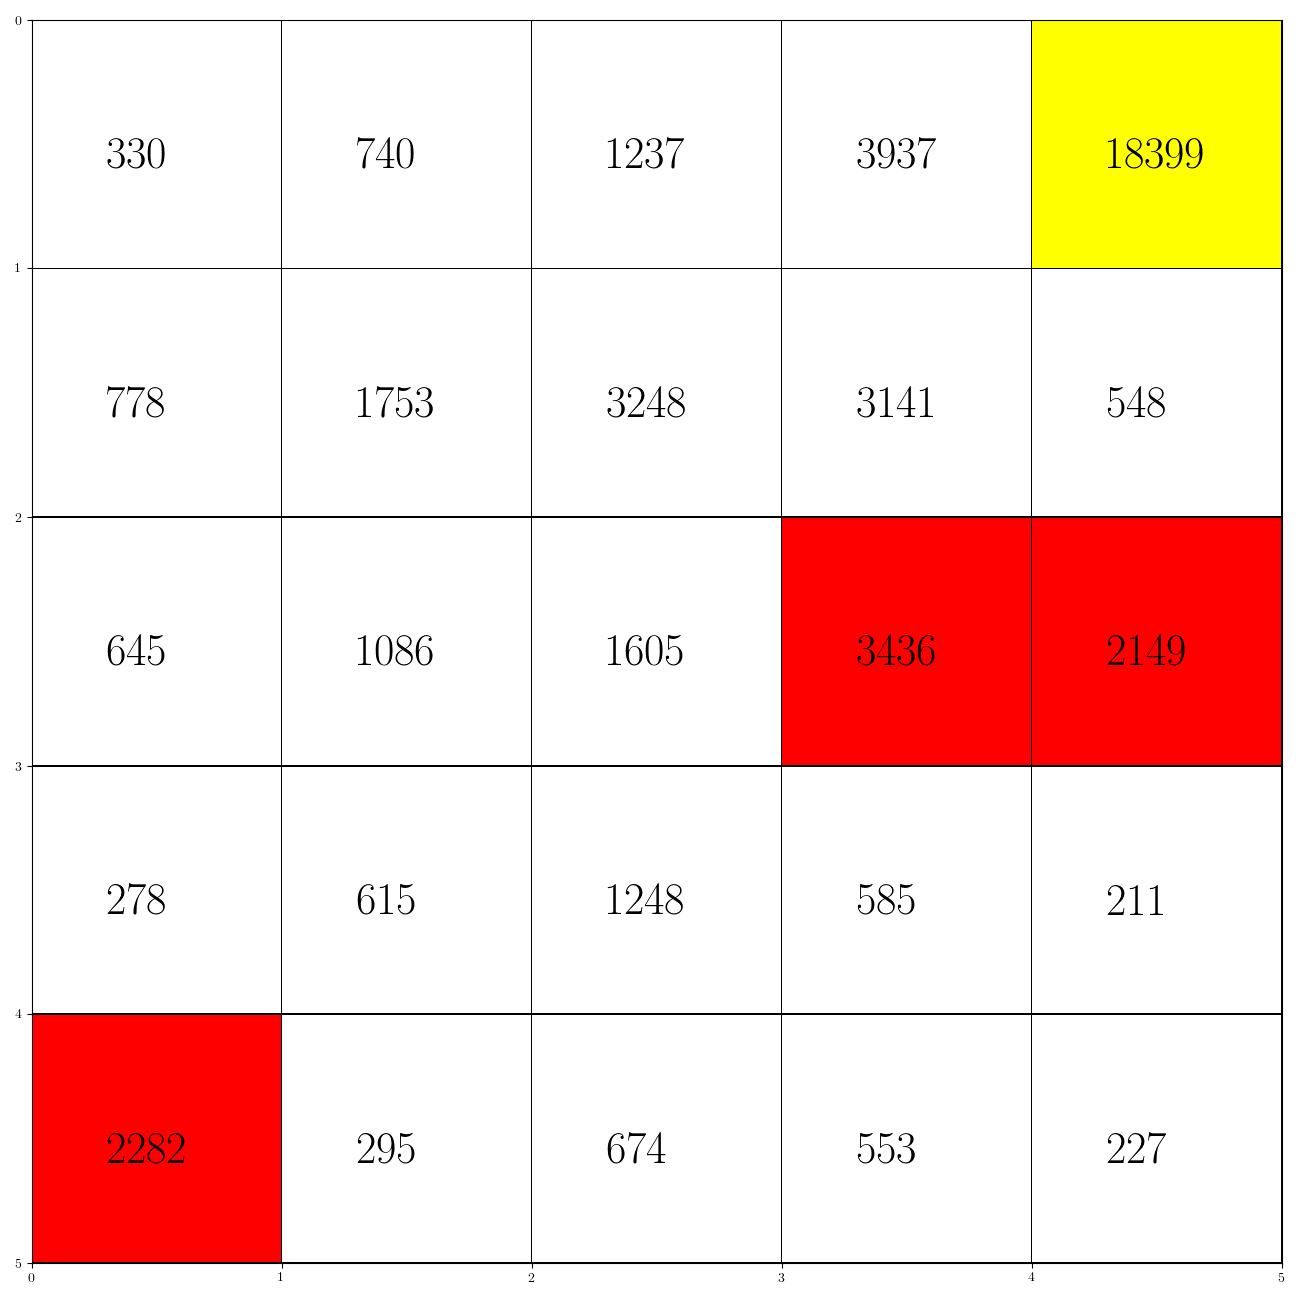
\includegraphics[width=\textwidth]{single_agent_demo}
                    \caption{State visitation count in single agent demonstration.}
                    \label{fig:single_agent_demo}
                \end{minipage}
            }

        \end{center}
    \end{figure}

\subsection{Experiment Hyper-parameters}
    To approximate the $Q$-function of \agent{2}, as described in Section \ref{sec:policy_parameterization}, let's start
    by placing a kernel centered at every grid cell. This sets $W=|S|\times A$, but it's a good test. See Fig.
    \ref{fig:kernel_visualization} for a visualization of how the the kernel function values, $k(s,a_2)$, at each state
    are mapped to the feature vector-function $\featFunc$. We'll set the following parameters:

    \begin{table}[H]
    \centering
        \begin{tabular}{c|c}
            $\kernStdDev_{\kernIdx}$ & $2.0,\ \forall l$ -- Identical kernel standard-deviations.\\
            $\kappa$ & $0.1$ -- Temperature of $\estimate{\policy{}}_2$. Eq. (\ref{eq:policy_model}). \\
            $\lambda$ & $1\mathrm{e}\!-\!4$ -- Gradient update rate. Eq. (\ref{eq:gradient_update}) \\
            $\eta$ & $0.2$ -- Gradient velocity memory.\\
            $m$ & 2000 -- Per iteration sample size of $\paramVec\sim \rho$.\\
            $\Lambda$ & $60$ - Moving average buffer length for $\mathsf{HIST}(\logLike)$. \\
            $\zeta$ & $0.001$ Gradient ascent termination when $\Delta\mathsf{HIST}(\logLike) < \zeta$.\\
            $\nu_{min}$ & $0.5$ -- Minimum parameter standard-deviation.\\
            $\nu_{max}$ & $1.2$ -- Maximum parameter standard-deviation.\\
        \end{tabular}
    \caption{Hyper-parameters used for single agent inference.}
    \label{table:single_agent_hyper_params}
    \end{table}

    \begin{figure}[h]
        \missingfigure{\Huge}
        \caption{Feature values for a kernel centered at cell $0$.}
        \label{fig:kernel_visualization}
    \end{figure}

\subsubsection{Algorithm bounds}

    There are often parameter elements that are not needed to maximize $\logLike(D|\rho)$. Sometimes, there are
    obviously extra parameters. In the case that \policy{2} is a hardmax, Delta Dirac, policy and we place a kernel at
    every state, there are $K+(|A|-1)$ unnecessary parameters. However, in the case when $D$ does not include data for a
    large subset of $S$ determining necessary must be done with care. We do not want to exclude a pivotal parameter that
    might be necessary to incorporate any future data, as we'll discuss in Chapter \ref{chapt:proactive_inference}.

    When a parameter \paramElem is not needed by the \textit{Q}-function approximation, \ie changes to this \paramElem\
    do not affect $\logLike(D|\rho)$. Naturally, the gradient dynamics of $\vect{\nu}$ in Eq.  \ref{eq:gradient_update}
    cause any unnecessary $\nu_{\paramIdx}$\!'s to grow indefinitely. This is a sampling complexity issue. As
    $\nu_{\paramIdx}$ increases, $ m $ must tend to $\infty$ at a much faster rate than the growth of $\nu_{\paramIdx}$
    to retain coverage of the assumed distribution. Sampling $\rho$ without enough coverage quickly causes
    $\logLike(D|\paramVec^{(i)}) \rightarrow -\infty,\ \forall\ i$. See Fig. \ref{fig:bad_gradient_dynamics_nu}.

    \begin{figure}[htb]
        \begin{center}
            \fbox{
                \begin{minipage}{0.75\textwidth}
                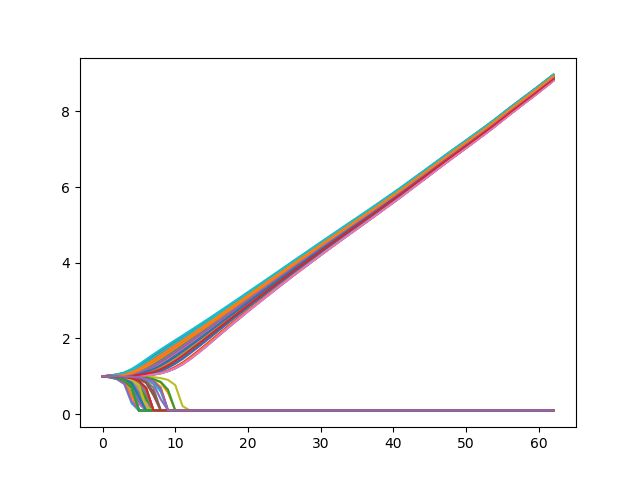
\includegraphics[width=\textwidth]{bad_grad_dynamics_nu}
                \caption{With unnecessary parameter elements, standard deviations grow uncontrolled.}
                \label{fig:bad_gradient_dynamics_nu}
                \end{minipage}
            }
        \end{center}
    \end{figure}


    \begin{figure}[htb]
        \begin{center}
            \fbox{
                \begin{minipage}{0.75\textwidth}
                    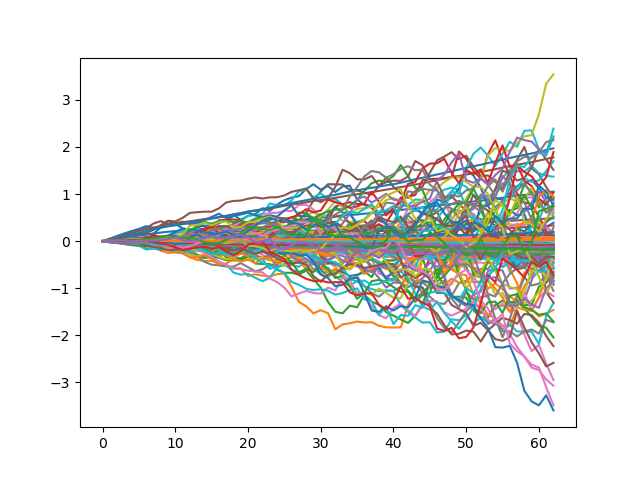
\includegraphics[width=\textwidth]{bad_grad_dynamics_mu}
                    \caption{With unnecessary parameter elements, some mean values grow uncontrolled.}
                    \label{fig:bad_gradient_dynamics_mu}
                \end{minipage}
            }
        \end{center}
    \end{figure}


    Similarly, even with a \textit{very} small gradient ascent rate, $\lambda \approx 1\mathrm{e}-6$, the necessary
    parameter elements have $\nu_{\paramIdx}$\!'s that quickly decrease in value and become invalid for any
    $\nu_{\paramIdx}\leq 0$. The remedy is to bound the covariance of $\rho_n$ with two more hyper-parameters,
    \begin{equation}\label{eq:param_var_bounds}
    \nu_{min} \leq \vect{\nu}_n \leq \nu_{max},\ \forall \nu_w \in \vect{\nu}_n.
    \end{equation}

    Thus, we add the last two hyper-parameters in Table \ref{table:single_agent_hyper_params}. Our Assumption
    \ref{assump:opt_policy_err} is verified by Figures \ref{fig:single_agent_logLike_25_kernels} and
    \ref{fig:single_agent_L1Norm_25_kernels}. The recorded $\mathsf{L}_1$-norm was neither used during gradient ascent,
    nor as a termination criteria. Note that the final $\mathsf{L}_1\text{-norm} \approx 0.01$. \color{blue} This final
    error has a range of about $[0.01-5]$ with these parameters over different trials.\color{black}

    \todo[inline]{
        Note that the legends in Fig. \ref{fig:single_agent_logLike_25_kernels} and Fig.
        \ref{fig:single_agent_L1Norm_25_kernels} are unclear.  In Fig. \ref{fig:single_agent_logLike_25_kernels}, the
        blue line is $\tilde{\logLike}(D|\vect{\mu}_n)$, the red line is $\max_{i \in
        m}\tilde{\logLike}_n(D|\paramVec^{(i)})$, and the green line is $\mathsf{HIST}(\tilde{\logLike}_n)$.  Similarly,
        in Fig. \ref{fig:single_agent_L1Norm_25_kernels}, the blue line is $\big|
        \OneNorm{\estimate{\policy{}}_{2}(s;\vect{\mu}_n)} -\OneNorm{\policy{2}(s)} \big|$, and the red line is $\big|
        \OneNorm{\estimate{\policy{}}_{2}(s;\paramVec_{max})} - \OneNorm{\policy{2}(s)} \big|$, where $\paramVec_{max} =
        \argmax_{\theta^{(i)} \in m}\tilde{\logLike}_n(D|\paramVec^{(i)})$.
    }

    \begin{figure}[htb]
        \begin{center}
            \fbox{
                \begin{minipage}{0.75\textwidth}
                    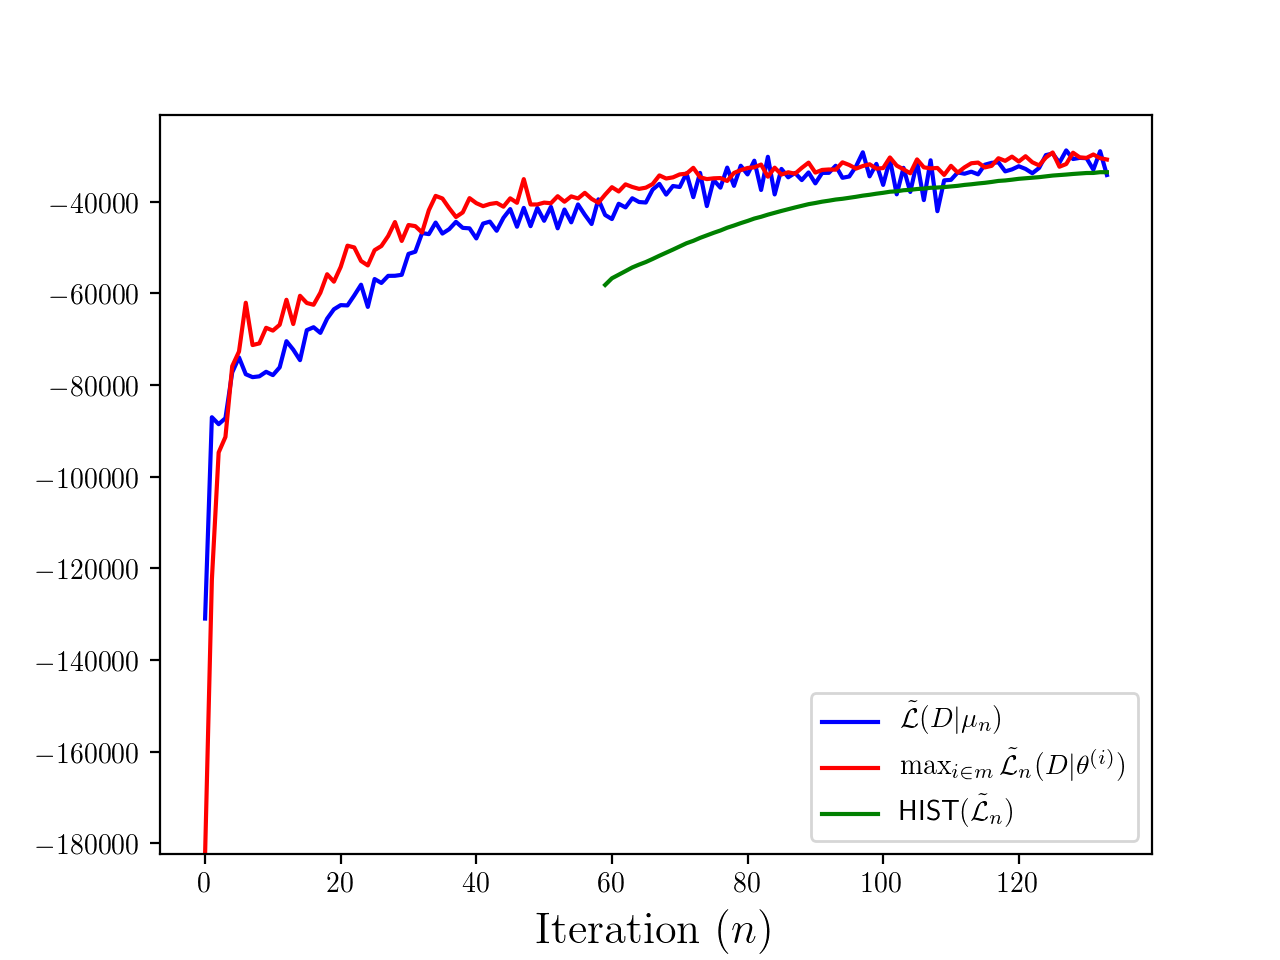
\includegraphics[width=\textwidth]{logLike_25K_temp_0_1}
                    \caption{$\logLike(D|\rho)$ with parameters in Table \ref{table:single_agent_hyper_params}.}
                    \label{fig:single_agent_logLike_25_kernels}
                \end{minipage}
            }
        \end{center}
    \end{figure}

    \begin{figure}[htb]
        \begin{center}
            \fbox{
                \begin{minipage}{0.75\textwidth}
                    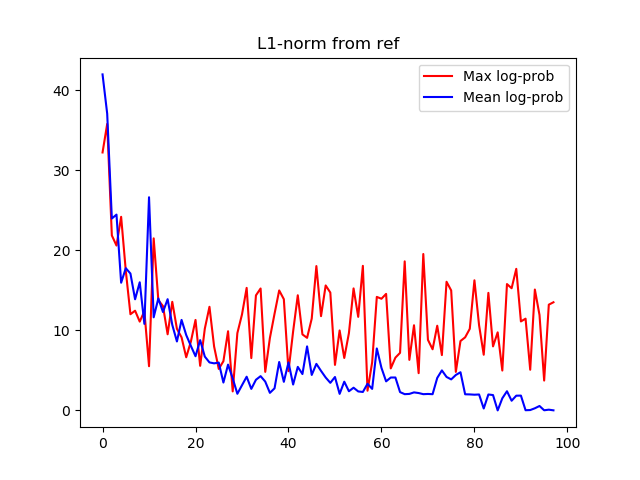
\includegraphics[width=\textwidth]{L1Norm_25K_temp_0_1}
                    \caption{$\big|\OneNorm{\estimate{\policy{2}}} - \OneNorm{\policy{2}}\big|$ with parameters in Table
                             \ref{table:single_agent_hyper_params}.}
                    \label{fig:single_agent_L1Norm_25_kernels}
                \end{minipage}
            }
        \end{center}
    \end{figure}
\todo[inline]{Perhaps change Fig 2.5 y axis to be fraction of maximum L1-norm?}

\subsection{Experiment with Fewer Kernels}

\todo[inline]{explain that blue circles are kernel centers.}
\color{blue} Note, not final discussion of results. \color{black}
New parameters are in bold. Isn't it interesting that the mean (blue) log-likelihood can still improve even though there
are no samples better than the log-likelihood of the current mean(Fig. \ref{fig:single_agent_logLike_9_kernels} compared to Fig. \ref{fig:single_agent_L1Norm_9_kernels})? (Happens independent of velocity-memory value). The distribution paramters are shown in Figures \ref{fig:smooth_gradient_dynamics_nu} and \ref{fig:smooth_gradient_dynamics_mu}.

    \begin{table}[H]
    \centering
    \begin{tabular}{c|c}
        $\kernStdDev_{\kernIdx}$ & $2.0,\ \forall l$ -- Identical kernel standard-deviations.\\
        $\kappa$ & $\mathbf{0.3}$ -- Temperature of $\estimate{\policy{}}_2$. Eq. (\ref{eq:policy_model}). \\
        $\lambda$ & $\mathbf{1\mathrm{e}\!-\!5}$ -- Gradient update rate. Eq. (\ref{eq:gradient_update}) \\
        $\eta$ & $\mathbf{0.2}$ -- Gradient velocity memory.\\
        $m$ & 2000 -- Per iteration sample size of $\paramVec\sim \rho$.\\
        $\Lambda$ & $60$ - Moving average buffer length for $\mathsf{HIST}(\logLike)$. \\
        $\zeta$ & $0.001$ Gradient ascent termination when $\Delta\mathsf{HIST}(\logLike) < \zeta$.\\
        $\nu_{min}$ & $0.5$ -- Minimum parameter standard-deviation.\\
        $\nu_{max}$ & $1.2$ -- Maximum parameter standard-deviation.\\
    \end{tabular}
    \caption{Hyper-parameters for smoother inference gradient dynamics.}
    \label{table:single_agent_new_hyper_params}
    \end{table}

    \begin{figure}[htb]
        \begin{center}
            \fbox{
                \begin{minipage}{0.75\textwidth}
                    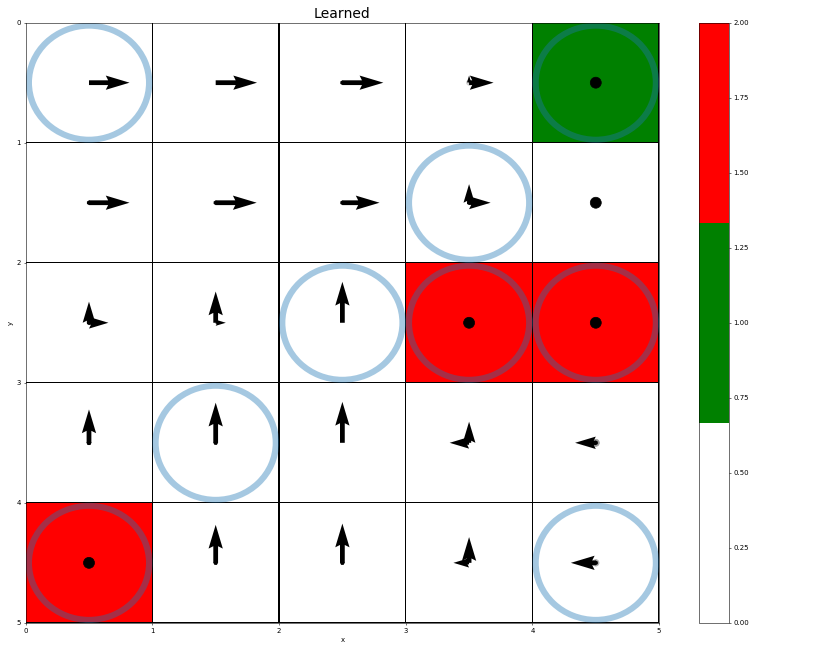
\includegraphics[width=\textwidth]{policy_9K_temp_0_3}
                    \caption{$\estimate{\policy{}}_{2}$ with parameters in Table \ref{table:single_agent_new_hyper_params}. The kernel in the green cell is very hard to see.}
                    \label{fig:single_agent_policy_9_kernels}
                \end{minipage}
            }
        \end{center}
    \end{figure}

    \begin{figure}[htb]
        \begin{center}
            \fbox{
                \begin{minipage}{0.75\textwidth}
                    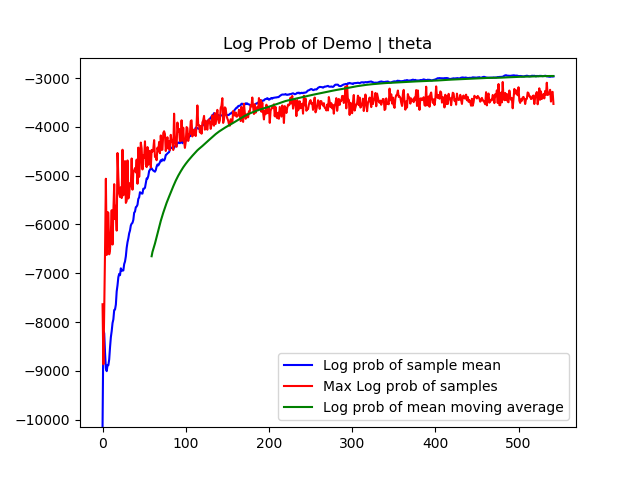
\includegraphics[width=\textwidth]{logLike_9K_temp_0_3}
                    \caption{$\logLike(D|\rho)$ with parameters in Table \ref{table:single_agent_new_hyper_params}.}
                    \label{fig:single_agent_logLike_9_kernels}
                \end{minipage}
            }
        \end{center}
    \end{figure}

    \begin{figure}[htb]
        \begin{center}
            \fbox{
                \begin{minipage}{0.75\textwidth}
                    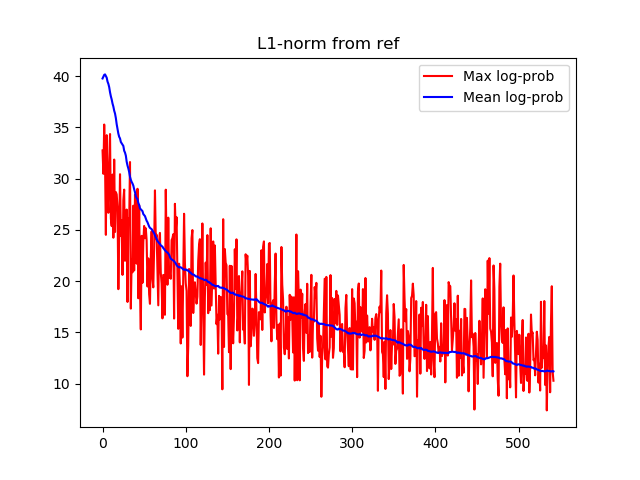
\includegraphics[width=\textwidth]{L1Norm_9K_temp_0_3}
                    \caption{$\big|\OneNorm{\estimate{\policy{2}}} - \OneNorm{\policy{2}}\big|$ with parameters in Table
                             \ref{table:single_agent_new_hyper_params}.}
                    \label{fig:single_agent_L1Norm_9_kernels}
                \end{minipage}
            }
        \end{center}
    \end{figure}


    \begin{figure}[htb]
        \begin{center}
            \fbox{
                \begin{minipage}{0.75\textwidth}
                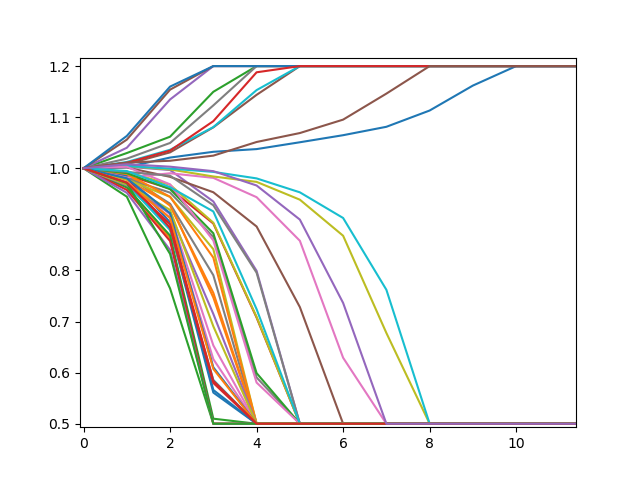
\includegraphics[width=\textwidth]{smooth_grad_descent_nu}
                \caption{$\nu_w$ for each iteration $n= 1,\ldots, 11$ with parameters in Table
                        \ref{table:single_agent_new_hyper_params}.}
                \label{fig:smooth_gradient_dynamics_nu}
                \end{minipage}
            }
        \end{center}
    \end{figure}


    \begin{figure}[htb]
        \begin{center}
            \fbox{
                \begin{minipage}{0.75\textwidth}
                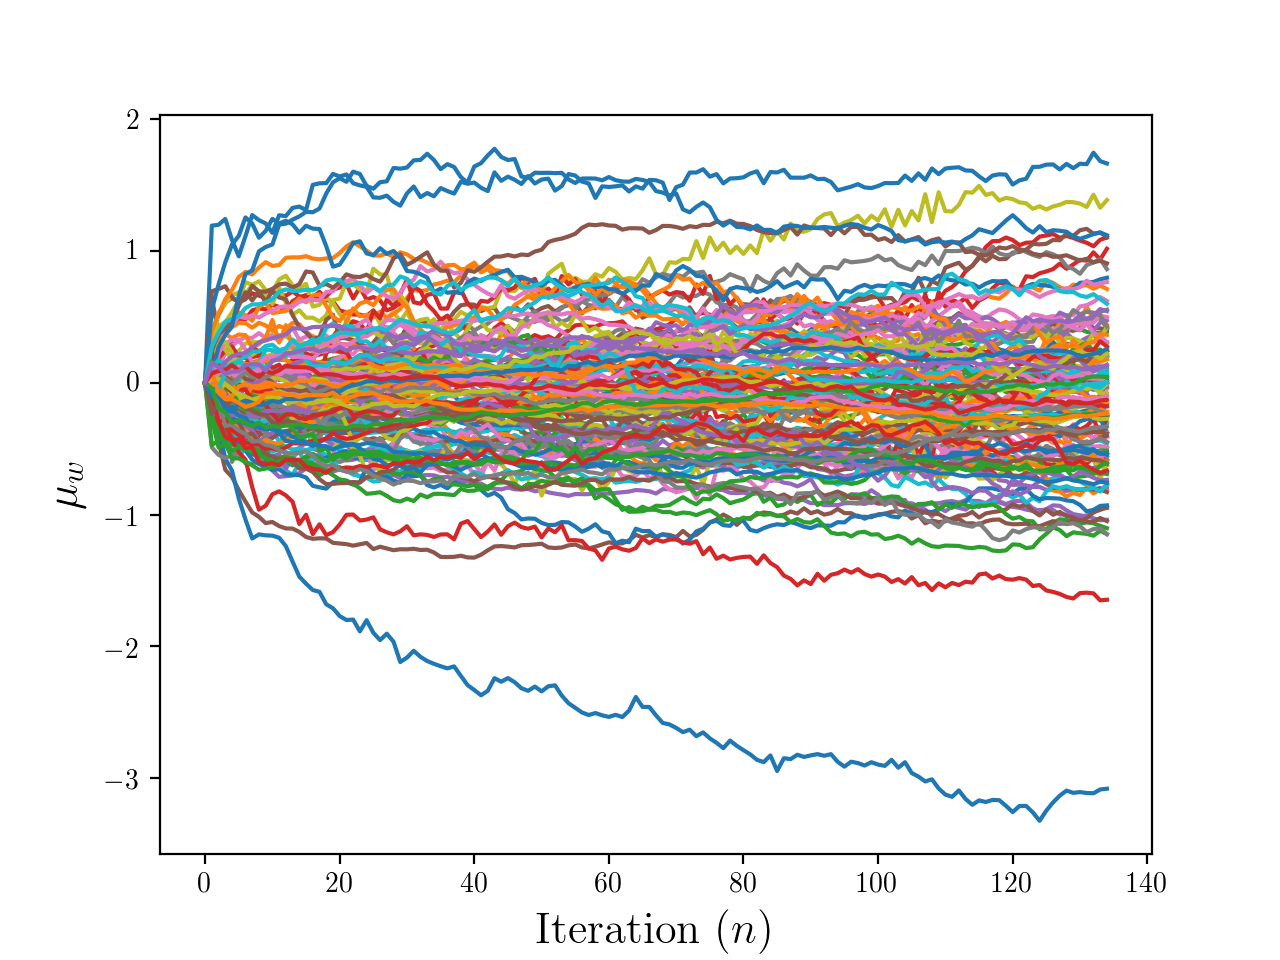
\includegraphics[width=\textwidth]{smooth_grad_descent_mu}
                \caption{$\mu_w$ for each iteration with parameters in Table
                        \ref{table:single_agent_new_hyper_params}.}
                \label{fig:smooth_gradient_dynamics_mu}
                \end{minipage}
            }
        \end{center}
    \end{figure}


    Note that if we use $K=9$, but use the parameters in \ref{table:single_agent_hyper_params}, we can achieve a final
    $\mathsf{L}_1\text{-norm} \approx 4.0$.

    \begin{figure}[htb]
        \begin{center}
            \fbox{
                \begin{minipage}{0.75\textwidth}
                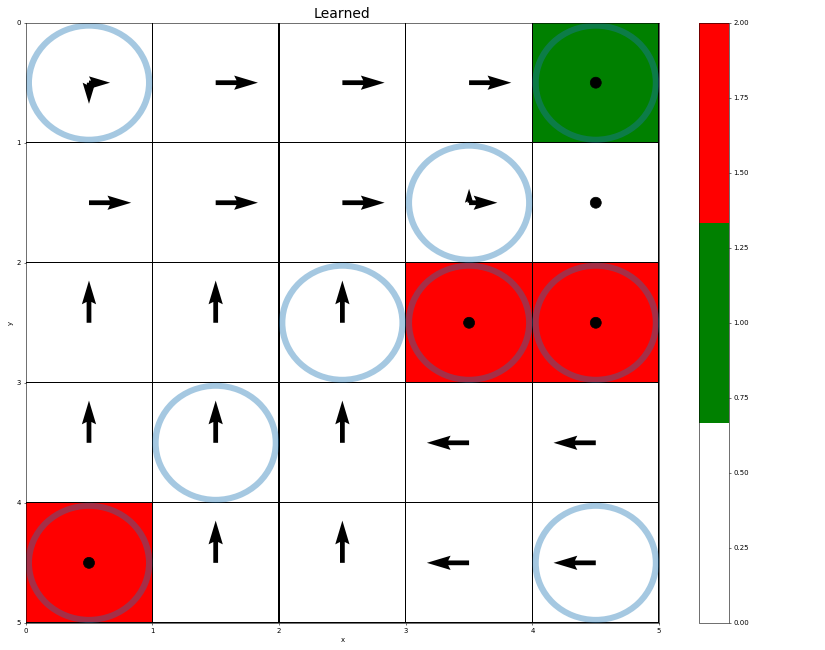
\includegraphics[width=\textwidth]{single_agent_policy_9K_fast_params}
                \caption{$\estimate{\policy{}}_{2}$ with parameters in Table \ref{table:single_agent_hyper_params}. The
                         kernel in the green cell is very hard to see.}
                \label{fig:single_agent_policy_9K_fast_params}
                \end{minipage}
            }
        \end{center}
    \end{figure}


    \begin{figure}[htb]
        \begin{center}
            \fbox{
                \begin{minipage}{0.75\textwidth}
                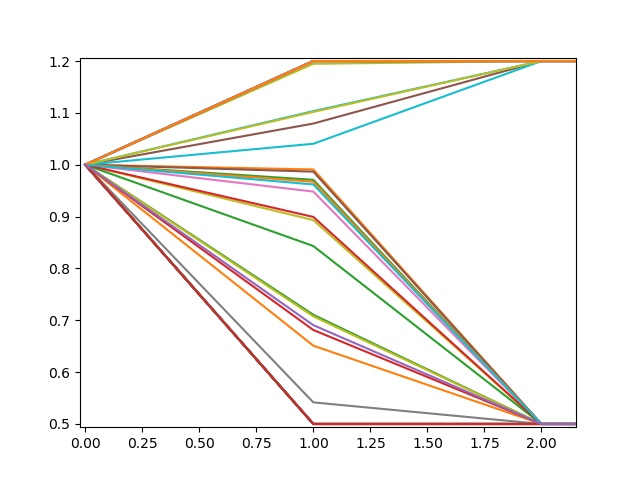
\includegraphics[width=\textwidth]{fast_grad_descent_nu_9K}
                \caption{$\nu_w$ for each iteration $n= 1,\ldots, 2$ with parameters in Table
                        \ref{table:single_agent_hyper_params}.}
                \label{fig:fast_gradient_dynamics_nu}
                \end{minipage}
            }
        \end{center}
    \end{figure}


    \begin{figure}[htb]
        \begin{center}
            \fbox{
                \begin{minipage}{0.75\textwidth}
                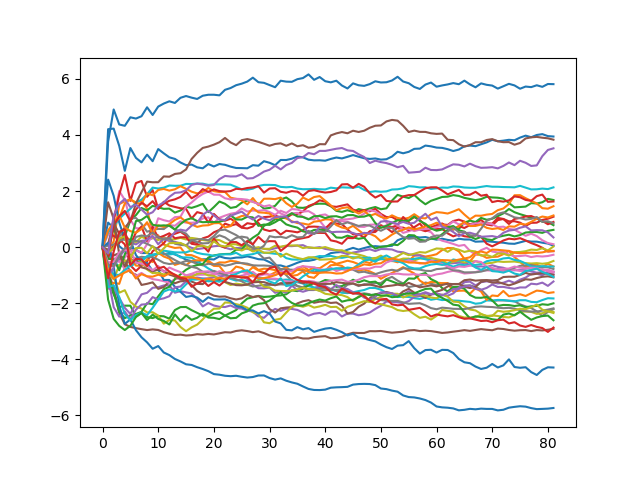
\includegraphics[width=\textwidth]{fast_grad_descent_mu_9K}
                \caption{$\mu_w$ for each iteration with parameters in Table \ref{table:single_agent_hyper_params}.}
                \label{fig:fast_gradient_dynamics_mu}
                \end{minipage}
            }
        \end{center}
    \end{figure}
